%\documentclass[conference,draftcls]{IEEEtran}
\documentclass[conference]{IEEEtran}

\usepackage{setspace}
%\doublespacing
%\onehalfspacing

\usepackage{ifpdf}
\usepackage[utf8]{inputenc}
\usepackage{cite}
\usepackage{paralist}
\usepackage[pdftex]{graphicx}
\usepackage{caption}
\usepackage{subcaption}
\graphicspath{{.}{images/}} 
\DeclareGraphicsExtensions{.pdf,.jpeg,.png,.jpg}
\usepackage[cmex10]{amsmath}
\usepackage{url}
\usepackage[rgb]{xcolor}
\usepackage{pdfcomment}

\usepackage{perpage} %the perpage package
\MakePerPage{footnote} %the perpage package comman

%\usepackage[tight,footnotesize]{subfigure}
%\usepackage[caption=false]{caption}
%\usepackage[font=footnotesize]{subfig}
%\usepackage[caption=false,font=footnotesize]{subfig}
%\usepackage{fixltx2e}
%\usepackage{stfloats}
%
%\usepackage[rgb]{xcolor}
%\usepackage{pdfcomment}
%\usepackage{geometry}
%\usepackage{marginnote}

\newcommand{\dme}[2]{\pdfmarkupcomment[markup=Highlight,color=yellow]{#1}{#2}}
\newcommand{\notedme}[1]{\raisebox{0pt}[0pt][0pt]{\pdfcomment[open=true,color=blue]{#1}}}
\newcommand{\todo}[1]{\pdfmarkupcomment[markup=Highlight,color=red]{#1}{todo}}

\newcommand*{\bd}[1]{\multicolumn{1}{|c|}{\bfseries #1}}


% correct bad hyphenation here
\hyphenation{op-tical net-works semi-conduc-tor}


\begin{document}
\title{Intrusion Detection within a Wireless Sensor Network Over the Air Update Protocol}
%The conference covers theory, design and application of computer networks and distributed computing and information systems
\author{
%	\IEEEauthorblockN{	A S M Ashraful Alam\IEEEauthorrefmark{1},  % and
%						David Eyers\IEEEauthorrefmark{1},  % and 
%						Zhiyi Huang\IEEEauthorrefmark{1} 
%					}
%	\IEEEauthorblockA{\IEEEauthorrefmark{1}Department of Computer Science, University of Otago, New Zealand, Email: \{aalam, dme, hzy\}@cs.otago.ac.nz} 
	\IEEEauthorblockN{	A S M Ashraful Alam,  % and
						David Eyers,  % and 
						Zhiyi Huang
					}
	\IEEEauthorblockA{Department of Computer Science, University of Otago, New Zealand, 
						Email: \{aalam, dme, hzy\}@cs.otago.ac.nz} 
}


\maketitle


\begin{abstract}
Security in Wireless Sensor Networks (WSN) is a challenging research area.
In this paper, an Intrusion Detection System (IDS) for a WSN software update protocol is modelled and simulated. 
The Intrusion Detection System (IDS) observes update behaviour effected by the Deluge protocol.
When Deluge modifies the running software in a mote, the mote sends related information to the sink. 
% <dme> I don't think the above is correct if using the omniscience approach that only works in the simulator
The IDS, in association with an IDS Transport Client (ITC) in the sink, analyses the update process and computes an `Intrusion Warning Score' (IWS) to indicate a possible intrusion i.e., a probable illegitimate software update.
\end{abstract}

% Note that keywords are not normally used for peerreview papers.
%\begin{IEEEkeywords}
%Wireless Sensors, WSN, Intrusion Detection System, Security, Intrusion
%\end{IEEEkeywords}

% no keywords
% For peer review papers, you can put extra information on the cover
% page as needed:
% \ifCLASSOPTIONpeerreview
% \begin{center} \bfseries EDICS Category: 3-BBND \end{center}
% \fi
%
% For peerreview papers, this IEEEtran command inserts a page break and
% creates the second title. It will be ignored for other modes.
%\IEEEpeerreviewmaketitle %not meant to be here for submission

%ICARA does accept papers on sensors. With collaborative robotics increasing rapidly, security of inter-robot communication over wireless media is of great importance. Your proposed paper would be of interest to ICARA attendees and we look forward to receiving your paper by 27th October.

\section{Introduction}
\label{sec:intro}
Wireless Sensor Networks (WSN) have seen much recent research.
They has attracted many researchers due to the significant advances in wireless and mobile communication technologies.
% <dme> such as?
The wireless sensors, which are also called motes or nodes, are generally battery-powered, embedded devices with a onboard radio chip and several sensors.
Sensors are deployed in the environment with a view to sensing certain physical phenomena, on which basic processing is performed at the individual motes.
The processed information is sent to the destination using a multi-hop relay mechanism for further processing.
The manager node, which is also called the sink or base station, generally has long-lasting power and is usually connected to a system with greater processing capability.
Motes operating within range, sharing the same protocols and radio channel form an autonomous network called a WSN.
A WSN does not have routers or gateways or routing tables.
% <dme> the sink is often thought of as a gateway AFAIUI, so the above sentence is potentially confusing.
It transports information using neighbourhood discovery process.
%\marginnote{Define mote, sink, WSN}[2cm]

Motes are generally deployed in a large number in uncontrolled environments, which makes them difficult to manage.
They are intended for long-term unattended use.
Once deployed, the applications in the sensors usually requires updating to accommodate bug-fixes, changes in sensing application or scientific requirements or alteration in the environment.
Network code propagation using over the air (OTA) data dissemination protocols provides a solution to this problem.
%\marginnote{Use of OTA Protocol}[2cm]

Protocols like Trickle, MNP, ReMo, Deluge and so on deal with OTA software update.
A few of the protocols facilitate preferential treatment at different subregions of the same WSN by allowing updating of a subset of nodes.
Most of the protocols update the  whole network at one go resulting into all nodes in the WSN running same updated version of the software.
For example, Deluge is an efficient and reliable protocol that allows OTA propagation of program binaries to all nodes in the WSN.
It addresses several network programming issues e.g., deals with program objects that can be larger than the sensor memory, works in environments with high packet loss rate, variable node density and asymmetric links \cite{1031506}.
It also ensures quick propagation of program codes with minimum service interruption, which make it an elegant protocol of choice for  WSN reprogramming to many researches and professionals.
Deluge is an interesting protocol to investigate any phenomena related to OTA reprogramming.
%\marginnote{OTA protocols -> Deluge}[2cm]

Security is considered an important aspect of WSN development due to the fact that  security threats to the WSN are different in nature from those faced when using Internet technology. % and ad-hoc network.
Unattended large-scale deployment makes WSNs an easy target to intrude upon.
Besides that, implementation of security techniques in WSN are critical and challenging because of constrained resources in the sensor.
Moreover, the capability of digital computing devices that can be employed to computationally compromise the security of sensors grows at an enormous pace in comparison to that of sensors.
% <dme> OK, but the sensors are gaining capabilities too...
In addition to that, WSNs have special vulnerabilities that do not exist in wired networks.
Wireless channels are inherently considered to be less secure.
Well developed secure mechanisms like WPS, PKM and likewise are inappropriate in WSNs. %WPS - WiFi Protected Setup and PKM - Privacy and Key Management for WiMAX
% <dme> you haven't said why they're inappropriate.
As a result, WSNs are more vulnerable to intrusion attempts and security threats from malicious attackers.
Besides physical attack on sensors, an attacker may also target wireless channels, network visibility, neighbourhood discovery process, and even the software update process itself.
Reliability and safety critics, and other researchers, have frequently pointed out that security issues in WSNs have not been sufficiently addressed, and that WSNs are not yet secure enough for deployment within mission critical applications.
%\marginnote{Security threats in WSN and reasond. Problem definition}[2cm]

%\subsection{Why WSN communication in robotics/any application need to be secured. }
%If inputs from wireless sensors are forged, then catastrophic errorneous results are expected			
%\subsection{Why it is important to secure updates? How WSN updates can be forged to impede the capabilities of robotics}


%\subsection{How do I plan to handle them (How do I do it). > Contributions} \\
In contrast to the problems described above, relatively simple communication protocols and the design of WSNs makes it easy to perform intrusion detection in them~\cite{quing09}.
An Intrusion Detection System (IDS) does not prevent the break-in, but it can detect  break-in events, and raise an alert following some predefined procedures in the case of a security breach.
Sometimes, it may be able to report the location and extent of break-in as well.
%Research in WSN security with respect to IDS has lots of potentials for new discovery and implementation. \empty{empty sentence}
In this paper we present an algorithm, which considers a centralised approach to detect  the intrusion in case of WSN software update.
The algorithm requires a minor modification of the OTA update protocol to send back a datagram e.g., an Active Message (AM) packet containing the update time.
AM is a single-hop, unreliable packet which are used to provide synchronous acknowledgements in TinyOS \cite{tep116}. %%It has a destination address, a type field, and a
%They are used to provide synchronous acknowledgements~\cite{tep116}.
%a message indicating update time.  %by incorporating Active Message (AM). 
%Specifically a TinyOS Active Message (AM) is used to acieve this. Such messages 
%AM is a single-hop, unreliable packet used for network abstraction in TinyOS. 
%It has a destination address, a type field, and are used to provide synchronous acknowledgements~\cite{tep116}.\notedme{The AM text still strikes me as weird. I've tried to rewrite it a bit. In a computer OS, if you wanted to say you sent back a datagram containing the update time, that's just what you'd say. It makes Active Messages sound like something special, when you haven't presented anything that's special about them. It's also not clear whether you're talking about the AM facility itself, or the data contained with the particular AM you send.} 
%<Ashraf>> I specified about AM because it is already an implemented datagram technique, which is handled by OS. One does not have to think about reimplemeting it, which need s special handling in different layers.
The information carried by the datagram enables the IDS with a centralised view of network-wide knowledge that is processed and analysed to work out a  `Surprise Score' or `Intrusion Warning Score' (IWS) to indicate a possible intrusion.
This work's contributions are two fold: 
\begin{inparaenum}
\item  The IDS identifies anomalies in software update patterns and scores them quantitatively;
\item It is demonstrated that simulation can indicate the positions of WSN nodes that will best support the ability of similar IDSs to detect anomalies.
%scheme i.e., the IDS expectations can provide useful insight for designing secure WSN.
\end{inparaenum}
%% <Ashraf> is this paragraph a repeatation of the previous one. But there are some useful info here
%\marginnote{Solution to the problem and contributions}[2cm]

%\subsection{Organisation of the paper }
The rest of this paper is structured in the following way. 
In Section~\ref{sec:lit}, we provide an overview of our findings from intrusion related research works in WSN. 
We seek software update security aspects not addressed by the present WSN security research and the reasons behind this. 
In Section~\ref{sec:meth}, we describe a brief overview of the system  design and the experiment methodology. 
Then we  present the findings from the experiments, analyse the result and present our evaluation in Section~\ref{sec:eval}.  
Finally, we conclude our arguments in Section~\ref{sec:concl}.
%\notedme{How many papers have you seen that have three sections? I'd expect five, usually.}
% <Ashraf>>I have given the details of structure asked by the conference committee in README file. For ICARA, they asked for three section actually and asked the Lit review to be included in intro.
%\marginnote{Paper Structure}[2cm]

\section{Background and Motivation}
\label{sec:lit}

%Data dessemination protocols
%Design of these networks to ensure the protection of data faces the constraints of limited power and processing resources. [REFERENCE: An Outline of Security in Wireless Sensor Networks: Threats, Countermeasures and Implementations]
The following section describes the background and motivation of the study.  It relates the effort to earlier research that has been performed in the field.


%% <Ashraf>> I am importing the rest portion from ICARA menuscript with comments from dme 
Software update process using Deluge or other OTA protocols is specifically vulnerable and a lucrative attack target because of several reasons.
First, the ability to infect a software update process implies effects beyond the updates only.
Secondly, most of the the OTA update protocols do not employ enough cryptographic protection for source authentication, integrity verification and likewise. 
The program binary authentication technique using a hash is not very useful in to resource-constrained sensors. 
Deluge incorporates digitally signed initial advertisement  and authenticated broadcast scheme. 
There is no mechanism to perform the integrity of the entire image object, because when the size of the object exceeds the size of available sensor memory, it becomes infeasible.
Additionally, a malicious intruder can replicate as an authentic image source and advertise new program version which the other motes cannot repudiate. 
%\notedme{This needs to be explained. It isn't convincing at the moment IMO.} %%<Ashraf>>>Tried to address
Thirdly, even though,  Deluge incorporates on-chip hardware based encryption, cryptography alone cannot prevent all attacks. %on WSNs confidentiality, authenticity, availability due to resource limitation.
Techniques of different types of attacks  on WSN have been described by \cite{DBLP:journals/corr/abs-1301-3022}.
Countermeasure  against these attacks are computationally expansive/costly and energy hungry, which implies that they cannot practically be employed in resource constrained sensors. 
Constrained computational capacity and resources make it possible to compromise the cryptographic measures incorporated in the implemented WSN OSs. \cite{aes2011}.  %\notedme{needs citation or other evidence.}
%%%Because the CC2420 cannot begin encryption at a particular offset and needs to be written, read, and re-written, use of the AES-128 may be  inefficient and will certainly decrease throughput. \cite{tep126}
Fourthly, an attacker can extract valuable information about the network from a physically compromised node.
He can utilise the knowledge to develop his attack strategy, even can replace the nodes with the illegitimate and malicious ones, which can imitate a legal update process. %\cite{DBLP:journals/corr/abs-1301-3022}.
Resource constraint, use of wireless medium, security-sensitive data, uncontrolled environment, distributed deployment and so on add to the physical vulnerability of the sensors.
Considering these reasons, some researchers strongly suggest complete redesign of security mechanism in WSN \cite{quing09}.
%\marginnote{Why OTA protocol is a potential attack target}[2cm]

While the OTA update protocols are essential for the WSNs, they may act as suitable carriers of malicious code in the network.
For example, Deluge achieves reliability using density aware epidemic property that works on a state machine principle and follows few local rules that ultimately achieves global behaviour \cite{1031506}.
If follows the other kind of vulnerability, which is breach at any one point weakens the whole WSN. 
This can result into complete compromise of the operations and functions of the WSN.
An attacker may appear somewhere in the network, pretend to be an authentic source and disappear after successful introduction of the illegitimate image to one mote in the network. 
The security mechanisms provided by Deluge would be unable to detect the initial breach in such cases and would allow the network to be flooded by a totally new version of the application that performs completely different function~\cite{Karlof:2004:TLL:1031495.1031515}.
%\marginnote{Ease of attacking OTA protocol}[2cm]

Protecting the software update process is certainly of great importance.
In case of failures, reporting such incidents and identifying the extent of illegitimate software update are also equally important.
During the software update process, the running OS needs to reboot to the new application. 
During this, security  measures on the sensor motes are deactivated or unavailable for a short period of time.
Additionally, the update process across the whole WSN contributes to a significant increase in traffic that an adversary may exploit to  mask his actions. 
With this end in view, an attacker can clandestinely initiate an illegitimate update and inject his own program image to serve his intended purpose.
This enables an adversary to steal sensitive information, log network events, even complete denial of service. 
%Researchers put lot of effort to study these attacks and to devise the methods to minimize their impact on the network.
%\marginnote{Why we need to protect the update process}[2cm]




%\subsection{Why it is necessary to have IDS not encryption in case of WSN}
Security schemes in WSNs have two main approaches -- using cryptography to secure communication and  employing IDS to oversee activities.
Cryptographic techniques are active approaches through use of cryptographic keys, encryption and decryption schemes, algorithms, policies and procedures.
Because  of the absence of the session and presentation layers in wireless sensors, applying encoding sockets and end to end encryption is impossible.
Designing cryptography based security solutions in the lower layers for wireless sensors are complicated, expansive and often may not be effective without being supported by additional measures from upper layers.
%\notedme{needs evidence} %<Ashraf>>Are you asking about the absence of the layers
An adversary can employ cryptanalysis with much greater computing resources to break in through the WSN cryptographic protection.
Moreover, absence of switches and gateways in WSN hampers monitoring of information flow.
Thus it is useful to employ some passive security measures, for example: an IDS.
Purpose of an IDS is to detect suspicious behaviour in the network, to provides useful information like identification and location of the intruder, extent of intrusion and likewise.
%\marginnote{WSN security mechanism}[2cm]


In recent years, researchers have suggested several intrusion or anomaly detection means to secure WSN, alongside the other cryptographic approaches.
The proposed techniques varies greatly in their idea and approach.
While some of them relies on deviation from statistical expectation of some phenomena, few of them also considers rule or policy based behaviours.
%\notedme{Why is there a need but not action? This seems odd...}
For example, an anomaly based IDS that works in a distributed manner and uses support vector machine to minimise communication overhead while performing in-network anomaly detection has been proposed by~\cite{ISI:000257882502160}.
A standalone rule based approach to detect anomalies at all layers of a network stack in WSN has been suggested by~\cite{1515559}.
Rule based  techniques rely on monitoring of group of nodes and routing tables for detection~\cite{ISI:000298891500099, Chen:2009:NMI:1516241.1516282, 1424814, Strikos_afull}.
On the other hand, spontaneous watchdog technique uses awareness about the sensor broadcast, density of deployed sensors for its detection~\cite{1593102}.
Specification based  IDS has been proposed that relies on data clustering and uses standard deviation from the average inter-cluster distance~\cite{Chen:2009:NMI:1516241.1516282, 4085803}.
%\notedme{What does this mean? Sounds almost exactly like what you're doing, no?}  
%<Ashraf>>The technique is Hierarchy based and depends on clusters. They use statistical measures. avoid statistical analysis?
Some anomaly  detection techniques look for anomalies in routing pattern and uses  hidden Markov model to decide on the accuracy of the gathered data~\cite{1290173, 4024996}.%\notedme{??} 
The model monitors data arrival process in real time traffic on the nodes, analyses short term dynamic statistics using a multi-level sliding window event storage scheme. % that works on each node. 
The detection algorithms performs locally and individual nodes are not aware of the network-wide attacks~\cite{1515559}.
%\marginnote{}[2cm]
An IDS based on game theory that also utilises Markov chains for its decision making, monitors only one of the network clusters at a time, which leaves the rest of the network unprotected.
The approach optimises the extra transmission or computation needed to defend by taking reactive approach in the game and assuming to be able to always identify the right cluster to defend using Markov chains~\cite{1347798, Das07preventingdos, Reddy:2009:GTA:1607720.1607944}.
%\notedme{why?}
%<Ashraf>>Mainly to preserve energy[extra transmission or computation needed to defend]. takes reactive approach on game.
Reputation based IDS relies on heuristic ranking algorithms to identify most likely bad nodes in the network.
Such IDSs use high scalable cluster-based hierarchical trust management protocol to effectively identifying the selfish and malicious nodes~\cite{6174485}.
In contrast, some other statistical procedures exploit the stability of the neighbourhood information of the WSN nodes depending on average receive power and average packet arrival rate~\cite{1512911}.
%\marginnote{Different types of IDS approach}[2cm]


Although very good results have been obtained from some of the approaches described above, only few of them are able to specifically address the security issues related to software update in WSN.
%\notedme{Evidence? The timing-based approaches sound like they'd work for addressing security issues in software updates...}
%<Ashraf>> None of the approaches described above uses time approach
The security countermeasures available in WSN systems is predominately cryptographic.
The WSN OSs do not incorporate an IDS approach due to the reality that deploying such software would cut down on the critical resources, especially power.
An IDS residing on the sensors ideally should be avoided by design.
%\marginnote{IDS desing issue}[2cm]

The absence of a passive approach to watch over the security breach of the software update leaves an easy back door  to intrude upon.
It is a threat to achieving authentication and integrity of information, maintaining confidentiality of the purposes for which WSN can be used.
Hence, we propose an analytical tool that is passive in nature and can provide valuable insight into the propagation characteristics of OTA reprogramming protocol. 
%\notedme{Although you need to contrast what you lose by not having it within the WSN.}
%The tool should be flexible for comparative studies of different protocols. 
%The tool, which is essentially an IDS, can primarily be applied on OTA protocol.\notedme{Weird sentence. What are you trying to say? It is an IDS, it is applied on OTA, what's your point?}
The technique has been tested on Deluge.
We have exploited services from other existing standard protocols to gather timing information from motes in  the WSN and then process the timing information for intrusion detection.
Use of timing analysis approach is a novel technique in IDS for WSN.
The IDS  resides outside the WSN and gathers processed information from the sensors in WSN.
%However, an IDS with that broad spectrum is out of scope of this paper.
%We shall limit ourselves within its application on WSN, specifically on Deluge only.
%Before one understands how the IDS works and is able to focus on its  mechanism, one needs some prior knowledge about Deluge and its security techniques.
The technique is controlled  centrally.
It  identifies anomaly in software update pattern in terms of quantitative score. 
The higher score indicates a higher probability of intrusion at some point in the WSN. 
The score can be deterministically classified when some additional information is available.
%\marginnote{Our proposition and rationale}[2cm]

%\notedme{What about the related work that talks about timing analysis?}
%<Ashraf>> I cannot find another timing analysis approach. And no IDS specifically addresses software updates. I was trying to identify IDS that talk about the software update issue
%The technique may further be extended for use with broad range of intrusion detection motives specially in WSN and also in MANET.
While timing analysis mechanism is non-existent in the WSN, some of the IDSs use traffic analysis or packet inspection  techniques.
It can be argued that traffic analysis approach is potentially comparable to proposed timing analysis.
The argument can be quite intense because traffic analysis considers both throughput and latency, and latency is essentially about timing.
Onat and Miri presented an IDS approach which considers statistical treatment similar to the one we proposed, yet the techniques have subtle differences.
The IDS deals with node impersonation and resource depletion attacks only.
In this approach, each node build an expectation statistics of received packets based on the last N packets received from each neighbour.
If packets received from any neighbour displays anomalous patterns after a predefined number of consecutive packets, intrusion alarms may be raised \cite{1512911}.
Unfortunately, the  packet count statistics is not suitable in OTA software update scenario.
There is a significant increase in packet traffic owing to software update process. 
This puts the mechanism off balance.
The other shortcoming of the technique is, certain rare yet critical activities, for example: a tsunami or earthquake, would raise false positive intrusion alarm.
However, the mechanism of statistical treatment on information over a time period motivates us to employ timing analysis approach on the context of OTA update protocol.
%\marginnote{Comparison with previous works. Motivation}[2cm]


\section{Methodology}
\label{sec:meth}
In this section, we provide a brief overview of the system design and describe the study environment and procedures.
The original system design is quite elaborate, but details have been left out to accommodate the space limitation.
%It's helpful to both writer and reader to organize this section chronologically: that is, describe each procedure in the order it was performed. For example, DNA-extraction, purification, amplification, assay, detection. Or, study area, study population, sampling technique, variables studied, analysis method.
The proposed IDS and its techniques were evaluated using a set of simulations. %in comprehensive simulations.
%While the system has been elaborately designed and aimed at testbed evaluation, it has not yet been performed at this stage of the research. 
%\notedme{Dropped sentence here. What does ``aimed at testbed evaluation'' mean?}
% <Ashraf>> I meant evaluation using a testbed implementation
%The testbed implementation will be evaluated at some point in the future.

%\notedme{You should redefine the term IWS in the body text I think. My rule of thumb is that you introduce abbreviations independently in the abstract and in the body text. Of course if you don't use an abbreviation subsequently, you shouldn't introduce it.}
%The raw data generated from simulation logs were processed, related and  analysed to produce the IWS.
%<Ashraf>>That is done now



\subsection*{System Overview}
\label{subsec:sysdeg}
The proposed IDS resides on an external computing system that is physically connected to the sink.
The system  relies on existing protocols for its operations.
Information necessary for IDS operations are collected utilising standard transport layer protocols. 
The IDS analyses the update time of  each of the motes in the WSN and computes IWS using utility function in Equation~\ref{eqn2} and indicates the cases of a possible intrusion, i.e., a probable illegitimate update.
The IWS, update time and image version information can be utilised to indicate location and extent of intrusion. 

The intrusion detection algorithm suggests some modification of the update protocol to enable an automatic reporting service in the mote by using AM packets to carry latest update information to the sink.
All motes in a WSN share a sense of time synchronisation which is accurate to 1~$\mu$s  and  is typically achieved using  TSMP\footnote{Time Synchronized Mesh Protocol devices e.g., motes stay synchronized to each other} protocol \cite{Pister08tsmp:time}.
The timing information carried by the datagram is therefore synchronised with other nodes in the WSN and can be used readily for processing by the IDS.

\subsubsection*{IDS Framework}
\label{ssc:ids_fw}
\begin{figure}[btp]
    \centering
    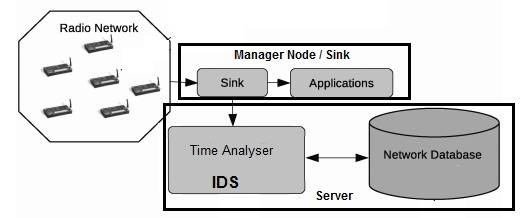
\includegraphics[width=0.5\textwidth]{IDS_fw}	
    \caption{IDS Framework}
    \label{fig:ids_fw}
\end{figure}
The IDS framework components and chronology of the activities associated with the IDS has been shown in Figure~\ref{fig:ids_fw}.
The IDS has three types of components:
\begin{inparaenum}
\item the motes in the WSN radio network that are subject to legitimate or illegitimate update e.g., intrusion attempt; 
\item an IDS transport client (ITC) application that runs on the sink and works in coordination with the IDS to assists in intrusion detection; and
%The sink is protected from all kinds of security breaches whether it is physical or logical. 
\item an IDS application that runs on a system with higher computing resources e.g., a server, which is physically attached to the sink, and houses a network database (NDB).
\end{inparaenum}

%%% <ashraf> strike out
%\begin{inparaenum}
%\item Updates are initiated using Deluge protocol;
%\item Deluge disseminates the new software image using the motes enroute to reach all the motes using a relay mechanism; 
%\item The nodes deliver their timing information to the sink using an AM packet;
%\item AM packets from the distant nodes rely on the other nodes enroute to reach the sink using a relay mechanism; and
%\item The ITC application in the sink delivers revelent information to the IDS for processing. 
%\end{inparaenum}
%The IDS analyses the acquired timing information to arrive at decision.
\begin{figure}[btp]
    \centering
    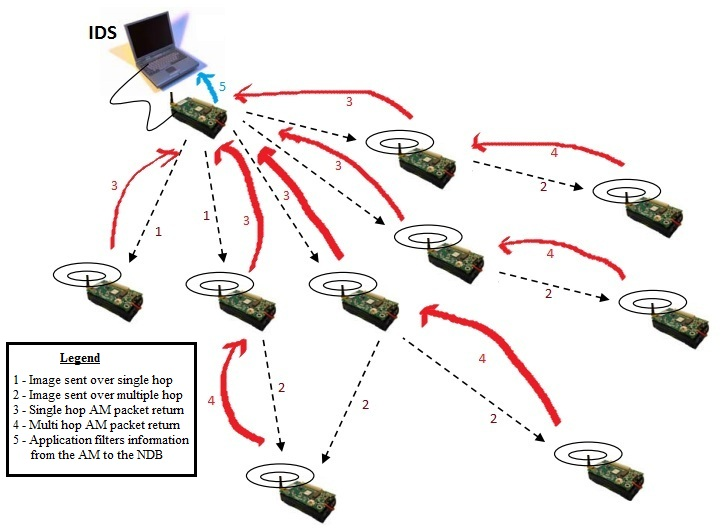
\includegraphics[width=0.5\textwidth]{IDS}
    \caption{IDS Modelling}
    \label{fig:ids_model}
\end{figure}

\subsubsection*{Determining IWS}
\label{ssc:cal_iws}
%% <ashraf> We cannot go into these details in this paper; space limitation
The intrusion detection activity begins with the action of motes by endorsing update time and initiating a datagram to the sink. 
%An AM packet initiated for the IDS has several fields: destination address, type identifier that indicates the update time information and the protocol for IDS, timing information and a checksum value.
%[DO WE WANT TO INCLUDE THE PATH TAGGING; MAY BE LATER - IT INCREASES RELIABILITY, NOT DIRECTLY $IDS$ ACTIVITY?]
%[path tagging is good, but in all cases, what’s the risk from intruders messing with the reported data?]
%[PATH TAGGING CAN BE USED AS HEART-BEAT MESSAGE]
The packet travels to the sink using a synchronous acknowledgement mechanism in transport layer protocols~\cite{tep116}.
%When it arrives at the sink, the checksum value is examined by the ITC to ensure that the packet content has not been altered enroute.
After checking for correctness, the ITC then inserts the update time, mote ID and related information to the NDB in the IDS.
The IDS maintains an identifier to differentiate among different update times from different runs for the same mote.
%
%The first software update run in the WSN is considered to be legitimate and the IDS takes this timing information as baseline.
%It is possible and desirable that the IDS is trained with several other update runs.
%More training improved the ability of the IDS to detect intrusion more accurately.
%Utilising multiple runs are useful and beneficial as it increases accuracy and dependency.
%However, the IDS needs to be manually controlled to enable multiple training runs.
%Outcome from these runs are statistically treated to build the baseline.

The authenticated initial software update runs are considered to be legitimate and the IDS takes these timing information to build its baseline.
The subsequent updates are liable to scrutiny by the IDS.
The time analyser module in the IDS inspects the NDB once an update activity has been detected.
It determines the changes in the statistics of the update time and calculates IWS based on following utility function:

\begin{equation}
\label{eqn2} 
	\mathit{IWS} = \sum \limits_{i=0}^{n} \frac{\left| \mu_i - t_i \right|}{\sigma_i + 1}
\end{equation}
where, 
\begin{inparaenum}
\item $\mathit{i}$---mote index;%\notedme{Why were you using capital letters all through here?} 
\item $\mathit{t_i}$---image update time at mote $\mathit{i}$;  
\item $\mathit{\mu_i}$---mean update time at mote $\mathit{i}$;  
\item $\mathit{\sigma_i}$---standard deviation of update time at mote $\mathit{i}$. 
\end{inparaenum}	

\subsubsection*{Building Intrusion Warning Zone}
\label{ssc:iw_zone}
The IDS can build a scale of possible expected range of IWS for a topology and can classify the IWS in different zones to imply certain warning levels.
While reporting severity or likelihood of an intrusion in quantitative term like the IWS is useful, it is more beneficial if the quantity is associated with some kind of interpretation.
The technique of associating such interpretation has been established by identifying Intrusion Warning Zone (IWZ) from a scale built from maximum expected IWS in a topology.
We have used a heuristic trial and error method to build the IWZ.
Threshold for building of Intrusion Warning Zone (IWZ) depends on the assumed ability of the IDS having IWS knowledge of all possible intrusions in the network.
%\notedme{This is not clear: you're jumping to talking about thresholds before describing what they are or why you want them.}
Such knowledge can be built by replicating intrusion activity from all nodes in the network.
In situations where it is not possible, replicating intrusion activity from the furthest few nodes may serve the purpose.
The heuristics follows from statistical techniques and feasibility of finding easily identifiable boundary.
%%<Ashraf>> I need to work more on this, I agree.
The IDS considers an IWS up to 10\% from the scale to be safe and marks as `GREEN' zone, an IWS above 30\% to be possible intrusion and is marked as `RED' zone.
%\notedme{Why? Where's the science here?}
However, an IWS within the range of 10\%---30\% can neither be considered safe, nor an intrusion, hence is marked as `GREY' to indicate a situation where rules are not known.
However, the thresholds are not conclusive and may require some variation based on the density, power level used in the WSN and scale of deployment.
%\notedme{This does not read strongly. It sounds like you're trying to make too much out of this: just state that for convenience of discussion, you define these zones. They seem entirely subjective to me: useful for discussion, but no more than that.}

\subsection*{Threat Model}
%What are the security aspects it does not handle?
%Why does not it handle them?

%\notedme{This is a start, but it's not very clearly written. Talking about the expected capabilities of attackers and vulnerabilities of the system would be good.}
The threat model is directed towards injection of unauthorised program image to infect the entire WSN.
The IDS is expected to handle malicious node update, node compromise, node failure.
In addition to this, the IDS also considers a threat model where a new node pops up and injects the new software image by compromising existing WSN security mechanism.
%The main threat scenario that the IDS is expected to handle is compromise of a particular node in the WSN and then attacker being able to utilise the same node or replicate the node to inject a new software image using Deluge protocol in the WSN.
%However, once the new image transfer has been injected, the node may remain alive or disappear.
%In case the compromised mote disappears, WSN would consider it as a node failure instead of node compromise.


An  attacker  can pickup one or more nodes deployed in hostile environment. 
He is able to access the code in a compromised node by employing superior computing power. 
In addition to this, he can also use cryptanalysis to gain this information even without compromising nodes physically.
Using the knowledge gained from compromised node, he can represent a false identity.
The attacker can also write his own or use existing protocols, utilise gained knowledge to initiate a software update to propagate in the network.
However, he has  no special  access to  the  network and is unable to modify the underlying protocols running in the uncompromised nodes.
%attacks  are  either  launched  from  compromised  sensor  nodes  running  malicious  code  or  unauthorised systems using stolen data (cryptographic keys & code) from legitimate nodes.
%Actually, the node was hijacked to infect the WSN and create more confusion in determining how the incident took place.
%\begin{itemize}
%\item Node failure
%\item Node compromise
%\item Malicious node update
%\item Popping up of intruder node
%\end{itemize}



%\subsubsection*{Assumptions} %Should I put it here or in discussio section.
%\label{sc:assump}
%\notedme{Misleading subsection heading---there are assumptions in other places, so make it clear which assumptions you're talking about.}

%Assumptions that are discussed in-text are discussed in the context of the limitations of your study, which is typically in the discussion section. This is important, because both assumptions and limitations affect the inferences you can draw from your study. - See more at: http://phdstudent.com/Choosing-a-Research-Design/stating-the-obvious-writing-assumptions-limitations-and-delimitations
%The system is expected to achieve a time synchronisation. 
%That's entirely reasonable, but it needs to be stated as an assumption about the WSN under study.
%I AM NOT SURE IF THIS PART IS AN ASSUMPTION> THIS IS A FACT.


The paper assumes several WSN settings and capabilities.
One of the most important assumption is single  sink scenario. While WSN with multiple sinks are also possible, the IDS needs to be designed differently and has not been studied at this stage of the research. 
It further assumes that the sink is protected from all kind attacks and cannot be compromised. 
The system do not consider mote mobility scenario and assumes a static WSN.
%The system operates in a fashion that whenever a new image updates a mote, it sends an AM to all the base stations in the WSN, thus the software update behaviour in the WSN is transparent to the IDS.

%The IDS is aware of the topological information that has been setup in the WSN.
%It knows the location of all nodes deployed in the network.
%I AM NOT SURE IF IT SHOULD COME AS ASSUMPTION. THIS IS ALSO A DESIGN ISSUE.
%However, assuming software update behaviour in the WSN transparent to the IDS enables fixing the scale for triggering warning.

%\begin{itemize}
%	\item	The WSN is of homogeneous nature and works in the same network.  - Too obvious
%	\item 	All motes in the WSN runs same version of the software.  - Too obvious
%	\item	IDS resides externally.  - A design issue, not an assumption
%	\item	There is A single sink in the WSN. 
%	\item	The sink is protected and cannot be compromised.
%	\item	Whenever possible, there are more than one route to reach each of the motes
%	\item	The WSN is static in nature- All motes in the WSN are static.
%	\item	Whenever a new image is updated in a mote, it sends a conformation active message to all base stations in the WSN, thus The software update behaviour in the WSN is transparent to the IDS.
%\end{itemize}

%\subsection{Algorithm}
%\label{subsec:alg}
%NOT STATED / DISCUSSED IN THIS PAPER\\
%This is a part in the original thesis though.




\subsection*{Experiment Settings}
\label{subsec:sim_env}
\begin{table*}[t!]
\centering
%\notedme{why is this table interesting or significant?}
%<Ashraf>> This is the result that I've presented
%\begin{tabular}{|l|*{8}{r|}r|}
\begin{tabular}{|p{2.5cm}|c |c |c |c |c |c |c |c |}
\hline
\bd{Topologies}           & \bd{Linear} & \bd{Circular} & \bd{Elliptical} & \bd{Double Rings} & \bd{Wide Line} & \bd{Grid} & \bd{Tree} & \bd{Owheo WSN}   \\
\hline
\bd{Number of Motes}           & 20 & 20 & 20 & 46 & 45 & 72 & 25 & 37   \\
% \bd{of Motes}           &  &  &  &  &  &  &  &    \\
\hline
\end{tabular}
\caption{Number of motes used in each topological deployment}
\label{tab:topos}
\end{table*}

The IDS requires Deluge protocol to be able to report the time of executing  a new version of its software.
The protocol was originally implemented in TinyOS and later has been ported to other embedded operating systems including Contiki\footnote{\url{http://www.contiki-os.org}}. 
We used Deluge protocol implemented in Contiki v2.7 on a system running on Ubuntu 12.04.
%[So this will eventually need citation and a self-contained description.]
`Cooja'\footnote{\url{https://github.com/contiki-os/contiki/wiki/An-Introduction-to-Cooja}}, a network simulator for Contiki, was used to simulate the software update pattern associated with Deluge protocol.
%\notedme{Best to give academic citations, or footnote URLs for these technologies.}
%We also used a plugin for Contiki called Mobility to aid our experiential setup.
%Although the plugin was designed to deal with positions over time for the nodes in the simulation, we used it to load the exact location of the sensor motes into the `Cooja' simulator. 

%\subsection*{Design of Experiments}
%\label{subsec:exp_des}

The simulation environment allows the software update pattern to be observed, by each WSN node reporting the time at which the new software update completes and starts executing.
The simulations evaluated the proposed IDS in different WSN topologies and explored the effect of parameters like power level.
%\notedme{Compare the commented and rewritten sentences here. Terms like `cautiously' are not useful unless the context is clear.} %<Ashraf>> Thanks
Evaluating the IDS on each of the topologies consisted of several test runs.
The test runs were of two kinds: 
\begin{inparaenum}
\item test runs aimed at establishing baseline data consisted of 20 individual simulations that were initiated from the sink; and
\item simulations that replicated intrusion initiated at different nodes except the sink.
\end{inparaenum}
Results obtained from all these simulations were utilised to model the expected pattern for a particular topology.
%
%\subsection*{Topologies}
%\label{subsec:topos}
The topologies were designed to observe the performance and effectiveness %of the  that were established using number of trial and error test runs 
of the proposed system in different environmental scenarios. 
In addition to this, effects of changes in parameters like power level on the IDS behaviour were also observed.
%\notedme{Not clear what you're talking about, specifically.}


%The shape of the experiential topologies were designed as linear, circular, elliptical, double rings, wide line, grid, tree and other random topologies.
%The names of the topologies here indicate that in each case the motes were deployed along the circumference of the geometrical shape that enabled packet propagation to take place according to a designed fashion.\notedme(1){drop---too obvious to justify saying.}
%In each topology, minimum 20 nodes were deployed for a test to take place. 
%More motes were necessary to replicate certain topologies.
Table~\ref{tab:topos} shows the number of motes used in experiments in corresponding topological  deployments.
The motes were placed at a distance of 30--35 meter to allow  multiple transmission paths to all motes. % <dme> en-dash for number ranges, not em-dash	% <ashraf> I am trying to increase my English and LaTeX vocabulary
For most experiments, the radio transmission power level was set at 100\% which has an approximate maximum effective transmission range of 50 meters and is able to interfere other motes upto 100 meters away.
The Owheo WSN topology was additionally tested at 50\%  to %quickly\notedme{?} 
observe the difference from the parameter change.


\subsection*{Procedure}
\label{subsec:proc}
%
%Experiment procedure  was a combination of activities such as running simulation, analysing system log and processing data to arrive at a conclusion. 
%\notedme{I'd just list the three steps if there are only three steps. Too simple to be worth using text to introduce subsequent short blocks of text.}
%
%
%\subsubsection*{Processing  of Individual Test Run}
%\label{ssc:test_runs}
%Step 1: Running simulation
\subsubsection*{Step 1} 
In the environmental set up described above , all motes in the WSN were booted up at same time running one version of a diagnostic application. 
The diagnostic application would necessarily report its time, version number and mote ID on the serial terminal every second at its serial port. 


%Step 2: Stopping the simulation
\subsubsection*{Step 2} 
The base station dynamically began the update process and propagated another version of the software image using Deluge protocol. %, which is also called 
Whenever the transfer to a mote was complete, the new image would replace its the one and reboot to begin executing itself.
The  new application necessarily initiates the motes to report their time, version number and mote ID on the serial terminal. 
In real system, the suggested modified Deluge protocol that runs with the OS would report the information to the sink using datagram.
The simulator continued until all the motes in the WSN were updated and the reported events were logged. 
%Step 3: Filtering out mote update time and distance
The update time of each mote were filtered out  and were sorted In ascending order of update time.

%Step 4: Calculating the euclidean distance and sorting
%A cpp application was used to take input from this semi-processed information and another file that preserved the position information of the motes in the deployment.
%The application processed the data to find out the euclidean distance of the motes from the sink.
%It additionally sorted the rows based on update time in ascending order.
%At this instance, we preserved the processed information in a file in following fashion:
%\begin{verbatim}
%--------------------------------------------
%| 	Time (in ms)	|	Mote ID	| Distance |
%--------------------------------------------
%\end{verbatim}

%Step 5: Calculating baseline data
%\subsubsection*{Building the Baseline Data}
%\label{ssc:build_baseline}
\subsubsection*{Step 3} 
To build the baseline for each topology, processed data from 20 simulations initiated from the sink were considered for building the baseline.
Any change in variable parameters or in the topology setup would necessitate recalibrating the baseline.
Mean and standard deviation of mote update times, generally in seconds, were statistically calculated to build the baseline.
These were the inputs to the IDS to calculate the IWS according to the utility function shown in Equation~\ref{eqn2}. 

%Step 6: Calculating IWS
%\subsubsection*{Calculating IWS}
%\label{ssc:calc_iws}

\subsubsection*{Step 4} 
Intrusion attacks at different nodes were replicated in simulations.
The individual simulations runs were treated in a fashion  similar to~Step 1 and Step 2.
The update time recorded at each of the motes were mathematically treated according to the utility function in Equation~\ref{eqn2}, which performed the following computations:
\begin{itemize}
\item Subtract new update time from corresponding mean of reference update time for each of the motes to calculate the absolute difference. For example, new update time of mote `$m$' is subtracted from mean update time found from the baseline data for mote `$m$' and its absolute value was calculated.
\item Absolute value is divided by a function of standard deviation to avoid division by zero situation. 
This is the intrusion score for individual node `$m$'.
%This also smooths the data to avoid unrelated variations.\notedme{what's an unrelated variation?}
\item Sum up the resulting intrusion scores at all individual nodes in the WSN to find out the total IWS for the update.
\end{itemize}
The resulting numbers  presented an approximation of abnormality of the new update pattern. The higher the score, the more dissimilar was the pattern. 


%\paragraph*{Step 6:} Calculating IW Zone / Classification


%\subsection*{Overview of the System}
%\label{sec:des}
%\notedme{...}



\section{Results and Evaluation}
\label{sec:eval}

\begin{table*}[t!]
\centering
\begin{tabular}{|l|*{20}{r|}r|}
\hline
\bd{Node ID}           & \bd{1} & \bd{2} & \bd{3} & \bd{4} & \bd{5} & \bd{6} & \bd{7} & \bd{8} & \bd{9} & \bd{10} & \bd{11} & \bd{12} & \bd{13} & \bd{14} & \bd{15} & \bd{16} & \bd{17} & \bd{18} & \bd{19} & \bd{20} \\
%Mote ID           & 1 & 2 & 3 & 4 & 5  & 6 & 7 & 8 & 9 & 10 & 11 & 12 & 13 & 14 & 15  & 16 & 17 & 18 & 19 & 20 \\
\hline
$\mu$            & 0 &19 & 19& 69&139 &213&276&344&377&432 &432 &432 &377 &335 &273 & 207&137 & 68 & 17 & 19 \\
$\sigma$		 & 0 & 5 & 5 & 6 & 22 & 36& 37&43 &44 & 44 & 44 & 44 & 44 & 45 & 44  & 33 & 24 & 5 & 3 & 5 \\
\hline
\end{tabular}
\caption{Time statistics of motes in Elliptical topology}
\label{tab:stat_ellip}
\end{table*}

%\begin{table*}[t!]
%\centering
%\begin{tabular}{|l|*{20}{r|}r}
%\hline
%\bd{Node ID}           & \bd{1} & \bd{2} & \bd{3} & \bd{4} & \bd{5} & \bd{6} & \bd{7} & \bd{8} & \bd{9} & \bd{10} & \bd{11} & \bd{12} & \bd{13} & \bd{14} & \bd{15} & \bd{16} & \bd{17} & \bd{18} & \bd{19} & \bd{20} \\
%\hline
%$\mathit{IWS}$
%                 &0.01&16 &19 &73 & 140 &203 &246 &336 &344 &396 &395 &535 &406 &332 &269 &237 &113 & 72& 16 & 16 \\
%\hline
%\end{tabular}
%\caption{Mote IWS in Elliptical topology. Further explained in Figure~\ref{fig:ellip}}
%\label{tab:iws_ellip}
%\end{table*}

\begin{figure*}[t!]
    \centering
    \begin{subfigure}[b]{0.5\textwidth}
        \centering
        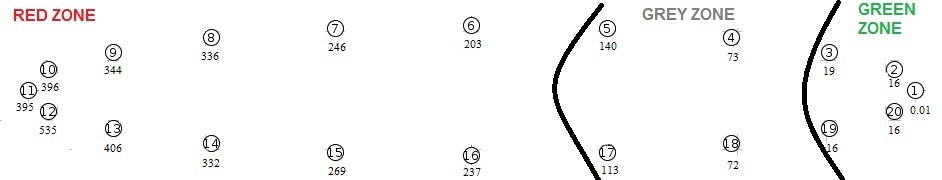
\includegraphics[height=1in, width=4in]{Elliptical}
        \caption{IWS and Relative position of nodes}
        \label{subfig:elliptopo} % <dme> it's is the \caption that updates the \label counters. You had \caption/\label in the wrong order.
    \end{subfigure}%
    ~ 
    \begin{subfigure}[b]{0.5\textwidth}
        \centering
        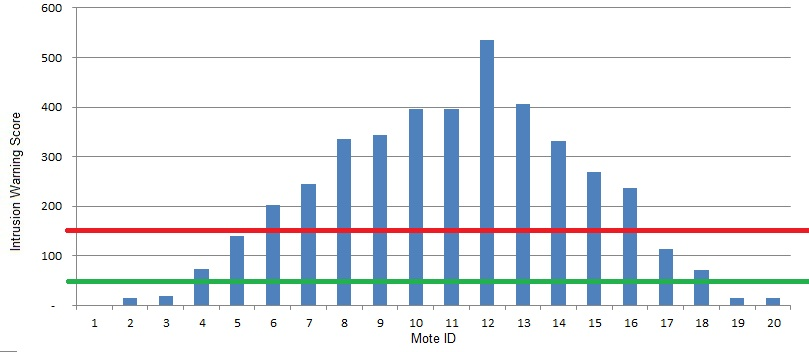
\includegraphics[height=1.2in]{Elliptical_column}
        \caption{Comparison of IWS at different motes}
        \label{subfig:ellipgraph} % <dme> it's is the \caption that updates the \label counters. You had \caption/\label in the wrong order.
    \end{subfigure}
    \caption{Relative position of the motes and comparison of IWS }
    \label{fig:ellip} % <dme> this was in the wrong place too
\end{figure*}

In this section, we presents the data found in the course of this investigation, their interpretation and evaluate the contribution.
While discussing the performance and effects of the proposed IDS in different topologies are useful, discussing any of the topologies presents fair idea about the outcomes from the others and mentioning the cases when the outcome was considered  contrary to the expectations.
The space requirement also motivates us to limit the discussion to necessary details only.


%\notedme{Put this earlier in the justification of discussing one topology in detail.}
%<Ashraf>> This is the second sentence in the discussion section
%\notedme(1){Is it closest to what you see in other papers? I'd not have thought so, in which case I'd think you need to justify why you're focusing on it... Also, there's unnecessary text repetition here.}
%% <Ashraf> The discussion is taken this way because of the spacew limitation and otherwise introducing all the results would be repeatation of the same thing, I guess. I'll look for papers that describe similar things.

%\subsection{Data1 + Discussion}

% We have selected data from elliptical topology for several reasons.
% Ellipse has a shape which is almost midway among the range of topologies between a circular and a linear one.
% Extending the minor axis of the ellipse makes the topology equivalent to a circle, while contracting it is equivalent to a grid or even a linear topology.
% Thickening the perimeter of the circle turns it into a double ring.
% Again, the linear topology can be considered as a tree with one or two branches.
% Extending it with more branches presents a fairly complex tree structure.
% Because of these similarities, discussing elliptical topology is an interesting choice.
%\notedme(1){Maybe...}
%% <Ashraf> removed because of space
we shall concentrate our discussion on results and findings elliptical topology only.
The ellipse shaped deployment of 20 nodes, as shown in Figure~\ref{subfig:elliptopo}, has been designed considering several requirements.
The motes on either side of minor axis remained within each others' transmission range, whereas motes on the either side of the major axis did not.
%Total 20 nodes were deployed with the minor axis being 30 meter and the major axis being way larger than that.
%The transmission power level was set at 100\%. 
% which allowed a  transmission range of 50 meter and nodes were  able to interfere other nodes at  up to 100 meter apart.
%The motes were placed at a spacing of 35 meters along the circumference of the ellipse to enable multiple transmission paths to all the motes.
It contributed to achieve  redundancy and  reliable image transfer. 

%The simulations proceeded without interruption and produced expected results.
% \notedme(1){This makes it sound like you're not going to present the results, which would be bad.}
% To build the baseline data, we assigned mote ID 1 as the sink and ran 20 updates initiated from the sink.
% The output from these runs were processed as describes in Section~\ref{ssc:build_baseline} and were statistically treated to compute the mean and standard deviation of the  time at which each of the nodes were updated with the new image.
%The computation results have been presented in Table~\ref{tab:stat_ellip}.
%\notedme(1){not yet clear enough what this table contains. Presumably `Node ID' should be explained to be the ID of the node from which to simulate injecting a malicious update so as to calculate the IWS? (+ broken ref)}
%% <Ashraf> restructured
Table~\ref{tab:stat_ellip} shows the baseline statistical measurements obtained at different motes.
The numbers indicate the measurements in time unit of seconds.
The first row in Table~\ref{tab:stat_ellip} contains the Node IDs that are headers for the data displayed underneath.
Node ID indicates the identification of each node in the deployment.
The next two rows describe the baseline data i.e., mean and standard deviation computed from the 20 legitimate updates initiated from the sink.
Analysing the baseline data shows that update time of the motes further away from the sink have higher mean and standard deviation.  
However, standard deviation raises gradually, though it varies little for relatively small distance difference when multiple paths are present.
The the stability of standard deviation results from availability of redundant paths, which makes the image transfer more efficient and reliable.
Therefore, even remaining at considerably different distances from the sink, mote ID 8, 9, 10, 11, 12, 13, 14 and 15  have quite similar standard deviation of update time.
In contrast to this, mean increases sharply as the motes are placed further from the sink.
The result in baseline data shows that motes closer to the sink have lower mean which follows a steep rise with the increase in distance.

Figure~\ref{subfig:elliptopo} shows the relative positions of the motes with mote ID written at the centre of the tiny circle and IWS beneath the circle.
IWS has been calculated using  the utility function shown in Equation~\ref{eqn2}.
Each of the motes were considered as intrusion point in the process of measuring IWS.
The IWS increases linearly with the increase in distance from the sink.
The `distance' term can be misleading without further clarification.
Euclidean distance between a mote and the sink does not make useful sense as the packets in the network must travel using a relay mechanism through other motes in the network.
Because of the availability of the multiple paths, it is not possible to quantify the exact distance that a packet would travel while transporting form a mote to the sink.
However, an estimation of distance along the most probable link path based on the connectivity may be considered.


IWSs shown in Figure~\ref{fig:ellip} were used to build a scale that ranged from $0$ to maximum of $\mathit{IWS}$.
Building this scale was crucial for the ability to classify the IWS to meaningful zones.
%\notedme(1){I thought that there were difficulties determining these zones?}
%% <Ashraf> I am not sure. Do you consider this description too simple?
It is not possible to build the scale without the knowledge of the expected IWS from the furthest nodes in the network.
Nevertheless, we used intuitive heuristics to classify zones  with two threshold levels at 10\% and at 30\%.
The IDS suggests different treatments for motes in different zones which are discussed bellow.

IWS is considerably higher for intrusion at distant motes than ones which are close to the sink.
This phenomena is topology dependent, which also implies  that it is connectivity dependent.
It is possible that if IWS in a network are organised in a specific order, it would represent/resemble   the original topology in some fashion.
For example, in the elliptical topology, the link path between node 1 and node 11 through node 5 is represented by a curve with a positive slope or rise.
On the other hand, the link path through node 15 is represented by a fall or a negative sloped curve.
There is a relationship between the curvature/eccentricity of the original topology and the represented curve or  trend.
%This implication would be more evident once we discuss more topologies in the upcoming paragraphs. {Only if we discuss the other topologies}.
However, establishing the relationship is beyond the scope of this paper.

IWS at different motes differ considerably: the motes close to the sink have very low IWS in comparison to the distant motes.
However, there are motes with IWS that can neither be considered low, nor too high.
These classes of scores inevitably demand different interpretation and treatment to indicate intrusion warnings. 
Accordingly, the Figure~\ref{subfig:elliptopo}  shows the region decided in GREEN, GREY and RED zones following to the technique discussed in Section~\ref{ssc:iw_zone}.
The graph in  Figure~\ref{subfig:ellipgraph} shows the relative measures of the IWS from the motes.
It also indicates the threshold among the GREEN, GREY and RED zones discussed above.

%\subsection{discussion of contributions}


\begin{table*}[t!]
\centering
\begin{tabular}{|l|*{20}{r|}r|}
\hline
\bd{Node ID}           & \bd{1} & \bd{2} & \bd{3} & \bd{4} & \bd{5} & \bd{6} & \bd{7} & \bd{8} & \bd{9} & \bd{10} & \bd{11} & \bd{...} & \bd{31} & \bd{32} & \bd{33} & \bd{34} & \bd{35} & \bd{36} & \bd{37} & \bd{38} \\
%Mote ID           & 1 & 2 & 3 & 4 & 5  & 6 & 7 & 8 & 9 & 10 & 11 & ...& 31 & 32 & 33  & 34 & 35 & 36 & 37 & 38 \\
\hline		\hline

Power	  &  &  &  &  &  &  &  &  &  &  &  &  &  &  &   &  &  &  &  &  \\
$100\% $          & 512 & 529 & 512 & 512 & 512  & 512 & 476 & 478 & 476 & 459 & 458 & ...& 49 & 47 & 53  & 48 & 49 & 51 & 47 & 29 \\
\hline

Power	  &  &  &  &  &  &  &  &  &  &  &  &  &  &  &   &  &  &  &  &  \\
$50\%$            &31 & 59&254& 31& 31 &283& 32& 32& 254& 31 &253 & ...& 31 & 31 & 31  & 30 & 31 & 31 & 30 & 0 \\
\hline
\end{tabular}
\caption{IWS from intrusion at motes in `Owheo Sensor Network'. Further explained in Figure~\ref{fig:owheo}}
\label{tab:owheo}
\end{table*}


\begin{figure*}[t!]
    \centering
    \begin{subfigure}[b]{0.5\textwidth}
        \centering
        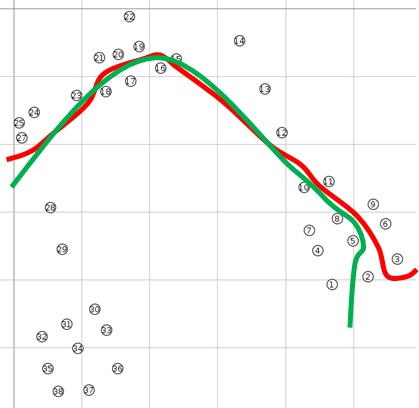
\includegraphics[height=2.5in]{Owheo_full}
        \caption{Zone boundary at Full Power Level}
        \label{subfig:owheo_full}
    \end{subfigure}%
    ~ 
    \begin{subfigure}[b]{0.5\textwidth}
        \centering
        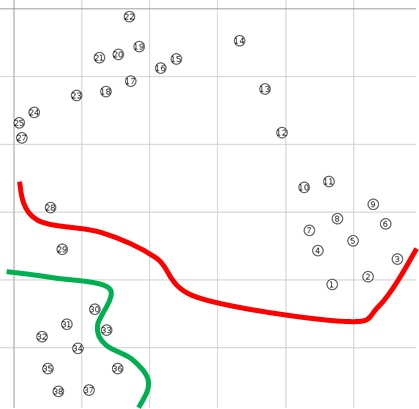
\includegraphics[height=2.5in]{Owheo_half}
        \caption{Zone boundary at Half Power Level}
        \label{subfig:owheo_half}
    \end{subfigure}
    \caption{Comparison of Zone boundary for power level variations in `Owheo Sensor Network'. IWS of the motes at the power levels are shown in Table~\ref{tab:owheo}}
\label{fig:owheo}
\end{figure*}

The main contribution of this research project comes from the fact that the IDS is able to report an anomaly from a software update in quantitative term like the IWS.
For example:  a regular legitimate update, initiated from node ID 1, resulted into a IWS of 0.01.
The result matched the theoretical expectation of a near zero IWS.
In addition to this, when intrusion scenario were simulated from the nodes near the sink, the IWS reported was fairly low, e.g. 16 for mote ID 2, 19, and 20
 and 19 for node 3 
 and likewise.
Because of the fact that IWS of the motes close to the sink are likely to be very low, which is in line with the theoretical expectation, it is quite difficult to conclude if such a IWS indicate an intrusion. 
However, for the distant motes, the IWS is quite high and the IDS can conclude such cases as intrusion, e.g. IWS of 246 for mote ID 7, 269 for mote ID 15, 395 for mote ID 11, 535 for mote ID 12 and likewise indicate intrusion.


While reporting severity or likelihood of an intrusion in quantitative term like the IWS is useful, it is more beneficial if the quantity is associated with some kind of interpretation.
The technique of associating such interpretation has been discussed in Section~\ref{ssc:iw_zone} and in this Section. 
In the elliptical topology intrusion scenario, maximum IWS reported in the data presented in Figure~\ref{subfig:elliptopo} was 535. 
Motes reporting 10\% of maximum IWS i.e., an IWS up to 53.5 would be considered in the GREEN zone.
%\notedme(1){Why is this the IWS value for green? You've not explained.}
%% <Ashraf> addressed
For example, in Figure~\ref{subfig:elliptopo}, mote ID 2, 3, 19, and 20 are in this zone.
On the other hand, IWS above 53.5 and bellow 160.5, which is 10\% -- 30\% of the maximum, are considered to be in the GREY zone. 
Motes in this zone are 4, 5, 17, and 18.
They can neither be considered free from intrusion, nor it is possible to easily arrive at a conclusion that the scores indicate intrusion for sure.
In contrast to both the scenarios describes above, IWS above 160.5, which is beyond 30\% of the maximum, is considered to be an intrusion.
All other motes in the topology have a IWS above this threshold level and hence are considered to be more easily detectable by the IDS. %\notedme(1){Eh? How does this follow?} %% <Ashraf> addressed

The idea of zoning associated with the IWS can be  very beneficial in securing a WSN.
It is useful in designing a secure network deployment, which is considered to be another major contribution of the research work.
%\notedme(1){`immensely' is too over the top.} %% <Ashraf> `immensely' removed
The motes which are found to be in the GREEN zone must be adequately secured by design with additional physical security as intrusion in these motes are not observed by the IDS.
%\notedme(1){OK, yep---I like this.} %% <Ashraf> addressed
On the other hand, motes in the GREY zone need additional monitoring which would aid determining if the IWS indicated a real intrusion or a false positive.
The additional monitoring could be in the form of an algorithmic or physical observation or listening post or even employing additional protocol.
The rest of the region, identified by the RED zone, is under the effective surveillance of the IDS and the IDS is expected give a reliable estimation of correct behaviour in this region.
%\notedme(1){not secure really, but yes, where the IDS can give a reliable estimation of correct behaviour}


A network is more secure when it has a smaller GREEN and GREY zone.
A smaller GREEN zone implies the requirement of lesser resources to impenetrably secure less number of motes.
Similarly, a smaller or non-existent GREY zone would require lesser monitoring measures.
Such a secure WSN can be designed by physically relocating some of the motes or even by varying the factors like power level.
However, obtaining real world scenario by varying different sets design parameters e.g., power levels, position of nodes, etc is an impossible task for even a small WSN.
The simulation environment used to design IDS can be effectively utilised to obtain expected IWS score range for different sets of parameters and then rank the sets based on how effectively they produce IWS values. 
For example, we have simulated the IWS scenario of the `Owheo Sensor Network'\footnote{`Owheo Sensor Network' is a WSN (mote ID 26 does not exist) deployed in the Department of Computer Science building at the University of Otago. It is intended to be used for research purposes.}
at two different power levels in our quest to design a secure WSN using the IDS.


%\notedme(1){I don't think you're quite stating the contribution clearly enough yet: that for different sets of potential design parameters for the WSN (e.g. power levels, position of nodes, etc.) you would be able to simulate the IWS score range, and rank the sets based on how effectively they produce IWS values. For example, it's not clear that your shift into discussing the zones is just an indirect way of discussing the underlying IWS scores.}
%% <Ashraf> addressed

Table~\ref{tab:owheo} shows the IWS at different motes as intrusion points at 100\% and 50\% power levels. 
In `Owheo Sensor Network', mote ID 38 was marked as the sink and.
At 100\% power level, 19 nodes (mote ID 1, 4, 5, 7, 8, 10, 16, 17, 18, 28, 29, 30, 31, 32, 33, 34, 35, 36, and 37) were in GREEN zone, only one node (mote ID 2) was in GREY zone and the rest 16 nodes were in RED zone.
The deployment and the zoning boundaries at 100\% power level has been shown in Figure~\ref{subfig:owheo_full}.
When the same deployment was simulated at 50\% power level, only seven nodes (mote ID 30, 31, 32, 34, 35, 36, and 37) were in GREEN zone, two nodes (mote ID 29, and 33) were in GREY zone and rest 27 motes were in RED zone.
The deployment and the zoning boundaries at 50\% power level has been shown in Figure~\ref{subfig:owheo_half}.
Comparing the scenarios presented in  Figure \ref{subfig:owheo_full} and \ref{subfig:owheo_half}, it can clearly be established that Figure~\ref{subfig:owheo_half}, i.e. deployment at 50\% power level is more secure than the other because of two reasons:
\begin{inparaenum}
\item it has a smaller sized GREEN and GREY zone; and 
\item there are fewer nodes in these zones. 
\end{inparaenum}
The deployment can be made more secure by physically relocating some of the motes from GREEN zone to RED zone, provided the relocation does not hamper the original intended purpose of the WSN.
However, any change in topology or design parameters like power level will require recalibrating the IDS from the beginning. 
%\notedme(1){I like this paragraph up to the last sentence. The last sentence doesn't make sense necessarily, since it seems to suggest that you can just move nodes directly between the zones. However any change in topology will require recomputing the zones, and they will change, potentially significantly...}
%% <Addressed>


%Identifying node failure and node compromise
The IWS is also able to detect node failures in the WSN.
%This additional advantage comes as a by-product contribution.
%However, as this was not a design consideration, the contribution is not robust enough, yet it is worth mentioning.
%\notedme(1){You've talked about this meta-point too much, now.}
%% <Ashraf> Actually, a `not' before `robust' went missing. :)
The case of a node not reporting its update time within a specified delay is handled by an error recovery procedure put in place by the IDS.
If the recovery procedure fails, the node is considered to have failed or have been compromised.
A unusual update time chronology and resulting unusual IWS  indicates the probability of some other types of attacks like node relocation, node repudiation, node compromise, not just a transient failure which is something worth paying attention to.
% However, such failure resulting into contribution towards an IWS which is quite different for the update pattern detected from the timing information reported by the other nodes.
% The IDS structure is such that it has an expected pattern and shape of IWS for an intrusion at some specific point.
% If the shape is distorted to a great extent, it indicates some unusualness which can be attributed to some other phenomena like node failure or compromise.
% The node failure or node compromise can take place concurrently with or without intrusion.
% It might also indicate a different type of attack associated with a physical intrusion.
% An interpretation form the IDS view of the topology would enable identification of some other types of attacks in WSN like node relocation, node repudiation, node compromise.
% \notedme(1){This paragraph probably needs to be much shorter. The point is simply that you're looking for a timing pattern, and that it involves a fair few transmissions. Thus if you see an anomaly, given that you're already comparing against a statistical distribution, it's probably not just a transient failure, and thus something worth paying attention to.}
%%<Ashraf> addressed

\section{Conclusion}
\label{sec:concl}

In this paper, we modelled an IDS solution to intrusion in WSN software update protocol.
We discussed the potential danger that is associated with WSN OTA software update protocol.
While OTA update protocols make certain WSN management tasks easy, they also remain vulnerable to intrusion attempts.
An adversary can take advantage of the resource constrained nature of the sensor motes and employ enough resources to break in through the limited protection the sensors are armed with.
To deal with this problem, we have suggested a passive security mechanism, an IDS.

The IDS is hosted on a server system that remains physically connected to the  sink. 
The sink has an ITC application which in coordination with the IDS performs the detection activity.
The system watches over the timing of software update pattern using a modified version of Deluge protocol.
Whenever a mote is updated, it sends an update related information to designated sink using a datagram.  
Related information from the datagram is filtered by the ITC for further processing at IDS.

The first contribution of the research is quantifying intrusion to an IWS that indicates the location and extent of intrusion.
The IWS is a quantitative indicator of possible intrusion.
The utility function that computes IWS is designed to neutralise the undesired %/unexpected
changes in mean and standard deviation which are expected to contribute to a near zero IWS.

The other important contribution is related to classifying expected IWS into zones.
The concept of zoning using the IDS is a very useful tool in designing secure WSN deployment.
The IDS can be used to simulate all possible combinations of parameters and  to rank the sets based on intrusion vulnerability.
For example, a WSN with known small insecure zone is much easier to protect than a larger zone.
The ranking mechanism is useful in such scenario.
Besides, the IDS also can indicate some other kinds of anomalies such as node relocation, node repudiation, node compromise and so on.

The IDS has several limitations. 
It assumes some special cases like static WSN with a single sink.
It also assumes to have network wide transparent knowledge.
These assumptions may not hold in real WSN.
In addition to this, assumptions about the attacker are: the attacker can employ enough resources to break in the cryptographic protections in sensors; however, he is not able to modify the protocols in an uncompromised sensor.
The IDS has an obvious functional limitation.
It cannot identify an intrusion in certain scenarios.
For example, when an intrusion takes place in close vicinity of the sink, this IWS may not always be significantly large to be identified as an intrusion.
The other limitation stems from the fact that the results are based on simulated data and needs support from real world implementation.
In future,  the IDS can be implemented to examine real world performance including cases of multiple sink with mobile sensors.



% Must explicitly state what is my contribution
% If there are some recommendations, must include them here
%What are my specific contributions to the academic society?
%Do I have some recommendations about it?



\IEEEtriggercmd{\enlargethispage{-5in}}

% references section
\bibliographystyle{IEEEtran}
\bibliography{aina}



% that's all folks
\end{document}


